\chapter{DOMAIN ANALYSIS}

Leak of centralize platform which gives student opportunity to post their thought and question, coupled with the limitations of the end-of-semester SIMU feedback system, restricts timely academic improvements and leaves prospective students with insufficient authentic information about university life.
\section{Problem Definition}

In Moldova, there is a significant gap in platforms that enable students to communicate,
share knowledge, and exchange experiences, unlike in other countries where
such platforms are common. The primary mechanism for student feedback, the
end-of-semester evaluation platform (SIMU), is limited to collecting feedback
once per semester without facilitating interaction or discussion among students.
This restricts timely improvements to the academic experience. Additionally,
students perceive a lack of anonymity in SIMU, fearing academic reprisal, which
discourages honest and constructive feedback. Furthermore, prospective students
rely on curated university marketing materials and anecdotal stories, which fail
to provide authentic insights into daily student life, leaving critical questions
about courses and campus experiences unanswered. A solution is needed to
create a platform that fosters continuous, anonymous, and transparent communication
and knowledge-sharing among students, enhancing the academic environment
and providing reliable information for prospective students.

\begin{itemize}
    \item \textbf{Infrequent Feedback Collection}: The SIMU platform collects feedback only once per semester, at its conclusion. This timing prevents instructors and administrators from implementing timely changes to address student concerns, rendering the feedback ineffective for improving the ongoing academic experience.
    \item \textbf{Perceived Lack of Anonymity}: Despite assurances of anonymity, many students fear that their critical feedback could be traced back to them. This apprehension, stemming from concerns about potential academic reprisal from professors, discourages honest and constructive criticism, undermining the quality and candor of the feedback provided.
    \item \textbf{Limited Information for Prospective Students}: Their primary sources are official marketing materials and anecdotal stories. While helpful, marketing content is designed to present the university in the best possible light and often fails to capture the day-to-day realities of student life. This leaves critical questions unanswered about course difficulty, professor teaching styles, campus culture, and the true student routine.
\end{itemize}

To address these challenges, our proposed solution, the Student Forum application, aims to provide a platform that facilitates continuous, anonymous, and transparent feedback from students. This platform will empower students to share honest insights and experiences in real time, fostering a more responsive academic environment and providing prospective students with a clearer, more authentic picture of university life.


\section{Problem Analysis}

To better understand the challenges students face and to validate the need for a
dedicated communication and feedback platform, we conducted a survey with university students across different years of study. The survey explored
frustrations during the semester, feedback practices, access to information,
and communication habits.

    \textbf{Frustrations During Semester:} \\
    Students most frequently reported difficulties with managing schedules and deadlines, 
    finding reliable study partners, and organizing group projects. These frustrations 
    highlight the need for a structured tool that simplifies coordination and improves 
    access to peer support.

    \begin{figure}[h]
    \centering
    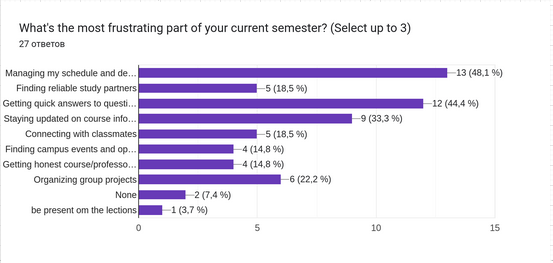
\includegraphics[width=0.8\linewidth]{img/survey/1sur.png}
    \caption{Most Frustrating Aspects of Current Semester}
    \label{fig:survey_results}
    \end{figure}

    As shown in Figure 1.1, managing schedules and deadlines (48.1\%) 
    emerged as the primary concern, followed by finding reliable study partners (18.5\%) 
    and getting quick answers to questions (44.4\%). These statistics reinforce the need 
    for a centralized platform that addresses these specific pain points.


     \textbf{Importance of Knowing Professors:} \\
    On a scale from 1 (not important) to 5 (very important), students rated an average of 
    around 4, indicating that knowledge about professors’ teaching styles significantly 
    influences their academic choices. However, most information is currently gathered 
    informally through word of mouth or social media, showing the lack of an official 
    and transparent source. \\

    \begin{figure}[h]
    \centering
    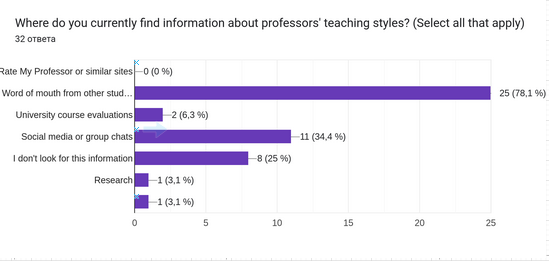
\includegraphics[width=0.8\linewidth]{img/survey/2sur.png}
    \caption{Sources of Information About Professors' Teaching Styles}
    \label{fig:professor_info_sources}
    \end{figure}
    

    As shown in Figure 1.2, word of mouth from other students 
    (78.1\%) is the predominant source of information about professors, followed by social 
    media or group chats (34.4\%). Notably, only 6.3\% of students use official university 
    course evaluations, highlighting the need for a more formalized and accessible platform 
    for sharing this information.

     \textbf{Barriers to Asking Questions:} \\
    A large portion of respondents cited fear of seeming unprepared, discomfort in 
    speaking up, or not wanting to waste others’ time as reasons for avoiding 
    questions in class or office hours. This demonstrates the need for anonymous 
    channels of communication where students can seek help without judgment.

     \textbf{Finding Academic Support:} \\
    Students typically identify helpful classmates by observing participation in class 
    or asking around randomly. This inefficient process shows potential for a platform 
    that makes peer expertise and study partnerships more visible and accessible.

    \begin{figure}[h]
    \centering
    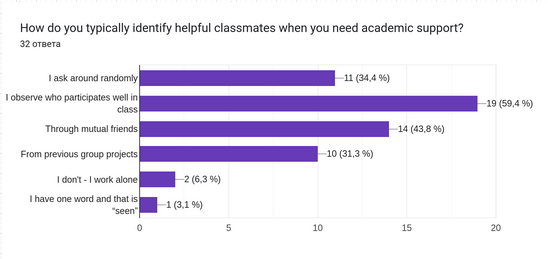
\includegraphics[width=0.8\linewidth]{img/survey/5sur.png}
    \caption{Survey Results: Methods of Identifying Academic Support Partners}
    \label{fig:academic_support}
    \end{figure}

    As shown in Figure 1.3, classroom participation observation 
    (59.4\%) is the primary method students use to identify potential study partners, 
    followed by connecting through mutual friends (43.8\%) and random asking (34.4\%). 
    Previous group project experience (31.3\%) also plays a significant role. Only 6.3\% 
    of students prefer to work alone, indicating a strong need for collaborative learning 
    support.


     \textbf{Communication and Coordination:} \\
    Most students rely on messaging apps and word of mouth to communicate with peers, 
    but these are fragmented and lack academic focus. Additionally, students reported 
    frequently missing important announcements or struggling to coordinate decisions 
    like meeting times, further reinforcing the need for a centralized forum.


    \begin{figure}[h]
    \centering
    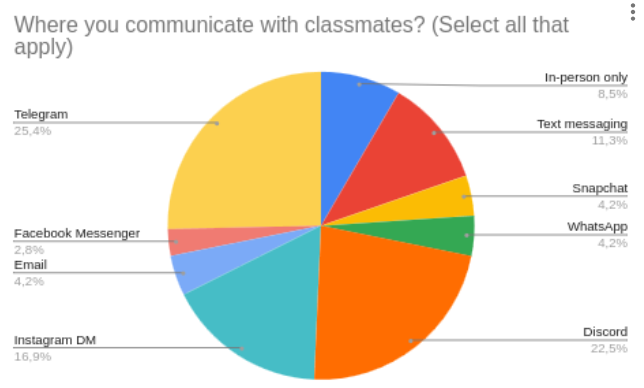
\includegraphics[width=0.8\linewidth]{img/survey/99.png}
    \caption{Primary Communication Channels Among Students}
    \label{fig:communication_channels}
    \end{figure}

    As shown in Figure, Discord emerged as the 
    primary communication platform, followed closely by Facebook Messenger and text 
    messaging. Email remains relevant for formal communications, while platforms like 
    Telegram and Instagram DMs are used by a smaller percentage of students. 
    Notably, in-person communication accounts for only about 11.3\% of interactions, 
    highlighting the strong preference for digital communication methods among 
    modern students.

     \textbf{Satisfaction with Current Tools:} \\
    When asked to rate satisfaction with existing tools on a scale from 1 to 10, the 
    average rating was low to moderate, signaling clear room for improvement in digital 
    platforms tailored to student needs.

    \textbf{Campus Events and Study Groups Discovery:} \\
    The survey investigated how students discover and stay informed about campus 
    activities and study opportunities. Results show a diverse mix of both digital 
    and traditional information channels.

    \begin{figure}[h]
    \centering
    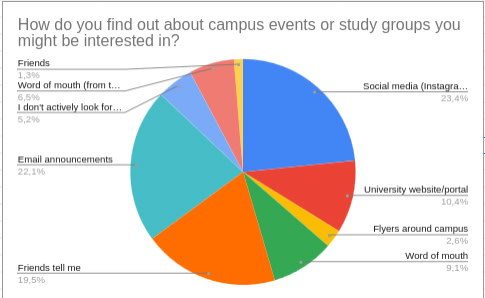
\includegraphics[width=0.8\linewidth]{img/survey/10sur.jpg}
    \caption{Survey Results: Sources for Campus Events and Study Groups Information}
    \label{fig:event_discovery}
    \end{figure}

    Social media platforms 
    (23.4\%) represent the primary source for discovering campus events and study 
    groups, followed closely by the university website/portal (22.1\%). Email 
    announcements (22.1\%) maintain significant relevance, while traditional methods 
    like flyers around campus (9.1\%) and word of mouth (9.1\%) still play a role. 
    Notably, 5.2\% of students report not actively seeking such information, 
    suggesting a potential gap in engagement that could be addressed through a more 
    centralized and accessible platform.



The survey confirms that students face recurring issues with communication,
feedback, and access to reliable academic information. Current solutions are 
fragmented, informal, and often discourage participation due to lack of anonymity. 
A dedicated platform would address these gaps by enabling continuous, transparent, 
and anonymous communication, ultimately improving the academic environment 
and empowering students with authentic insights.




\section{Solution Proposal}

Based on the survey results and identified challenges, we propose the development 
of a \textbf{Student Forum Platform}. This solution directly addresses the needs 
of both prospective and currently enrolled students by providing a centralized, 
anonymous, and transparent space for communication, feedback, and knowledge-sharing. 
The following arguments illustrate the necessity and impact of this platform.

\subsection{Argument I: A Platform for Prospective Students}

\textbf{The Problem.} 
Prospective students are often forced to make one of the most important decisions 
of their lives---choosing a university---based on limited and idealized sources 
of information. Their primary references are official marketing materials and 
anecdotal stories. While helpful, these materials are curated to present the 
university in the best light and rarely capture the realities of daily student 
life. As a result, important questions regarding course difficulty, professors’ 
teaching styles, campus culture, and the overall student experience remain 
unanswered.  

\textbf{The Consequence.}  
This lack of authentic information creates uncertainty and hesitation. Prospective 
students who cannot find genuine, peer-to-peer answers to their concerns may feel 
less confident in their choice and may opt for other institutions that appear more 
transparent and relatable.  

\textbf{Our Solution.}  
The forum will offer a dedicated, searchable space where prospective students can 
directly ask questions to the university community. Current students can share 
their genuine experiences, providing an unfiltered perspective on courses, 
professors, and campus life. This peer-to-peer interaction creates a trusted and 
transparent resource, empowering prospective students to make more informed 
decisions and increasing the likelihood of their enrollment.

\subsection{Argument II: A Platform Where Enrolled Students Are Heard}

\textbf{The Problem.}  
For enrolled students, satisfaction and belonging are critical to their academic 
success and retention. However, the existing feedback system is inadequate. The 
current mechanism, the SIMU platform, suffers from two major limitations:
Feedback is collected only once at the end 
    of the semester, when it is too late to implement meaningful improvements.  
 Despite assurances, many students 
    believe their feedback is not truly anonymous. This fear of academic reprisal 
    discourages open and constructive criticism.  

\textbf{The Consequence.}  
This flawed feedback system creates an environment where students feel powerless 
and unheard. Unresolved concerns about teaching quality, course design, and 
administrative practices accumulate over time, leading to frustration, 
disengagement, and in some cases, student attrition.  

\textbf{Our Solution.}  
The proposed forum provides a continuous, community-driven dialogue space where 
students can openly discuss academic and administrative issues in real time. 
Anonymous participation ensures that students feel safe sharing candid feedback 
without fear of reprisal. Beyond individual expression, the platform fosters 
collaborative problem-solving, allowing the student body to collectively identify 
issues and propose solutions. This cultivates a stronger sense of agency, 
involvement, and ownership in the academic community.  

By addressing the needs of both prospective and current students, the Student 
Forum platform creates a dual impact: it strengthens the university’s reputation 
and attractiveness for future applicants while simultaneously enhancing the 
academic environment for those already enrolled. This solution fosters 
transparency, trust, and collaboration, ultimately contributing to a more 
supportive and dynamic university community.

\begin{table}[h!]
\centering
\caption{SWOT Analysis}
\begin{tabular}{|p{5cm}|p{3.5cm}|p{3.5cm}|p{3.5cm}|p{3.5cm}|}
\hline

\textbf{Strengths} & \textbf{Weaknesses} & \textbf{Opportunities} & \textbf{Threats}  \\
\hline
Most comprehensive features set& Resource - Intensive & Potential Partnerships & Resistance to change from other social media \\
\hline
Flexible group/channels system & Limited Accessibility of user accountsfrom university &  Feedback and improvement in real time & Competing Solutions   \\
\hline
Freandly UI& No anonymity features & University community chat & Connect all university in one app   \\
\hline 
University multiple content type& Privacy content & Ditch the teacher for better learning & Motivate people to use our app  \\
\hline
\end{tabular}
\end{table}

\section{Target Group}

The target audience includes two different groups: \\
\textit{Students:} Students are the primary target group. 
They are involved in following aspects:Undergraduate and graduate students seeking academic support. 
Students looking for study groups and project collaborators. 
Those wanting to share experiences about courses and professors. 
Students seeking real-time feedback and answers to academic questions \\

\textit{Potential Students:}
High school graduates researching university programs. 
Transfer students evaluating the university environment. 
International students seeking authentic insights into campus life. 
Individuals exploring specific course experiences and requirements 


\section{Existing Solutions}

The landscape of student-focused social platforms has evolved significantly in recent years, driven by changing communication preferences and the increasing digitization of academic communities. This comprehensive analysis examines four distinct platforms that serve various aspects of student social interaction and community building. The platforms under consideration include the berkslv social media application, GoIn Connect's pre-enrollment community platform, Jodel's anonymous hyperlocal network, and the proposed student forum solution designed with Reddit-like functionality.

Each platform addresses unique market segments within the broader student community ecosystem. The berkslv application focuses on verified Turkish university students through institutional email verification, creating a trusted regional community. GoIn Connect operates in the pre-enrollment space, facilitating connections between admitted students before they arrive at universities, with a business-to-business model targeting educational institutions. Jodel provides anonymous, location-based social networking within a 10-kilometer radius, appealing to students who prefer privacy in their digital interactions. The proposed student forum aims to combine the familiar Reddit interface with student-specific features including channels, polls, and category-based organization.

The analysis reveals significant opportunities in the market for a platform that can effectively combine the strengths of existing solutions while addressing their limitations. The proposed student forum platform has the potential to occupy a unique position in the market through its comprehensive feature set and focus on long-term academic community building rather than ephemeral social interactions.

\section{Platform Functionality and Core Purpose}

\subsection{berkslv Social Media Application}

The berkslv social media application functions as a closed social network exclusively designed for Turkish university students. The platform operates on the principle of verified academic communities, requiring users to authenticate using official university email addresses ending with .edu.tr domains. This verification system ensures that all participants are legitimate members of Turkish higher education institutions, creating a trusted environment for academic and social discourse.

The application serves as a digital campus commons where Turkish students can share experiences, discuss academic matters, and build connections within their national higher education community. Users can create posts about university life, academic challenges, career opportunities, and social events relevant to the Turkish student experience. The platform facilitates connections between students from different universities across Turkey, enabling knowledge sharing and collaborative opportunities that might not otherwise occur.

The focus on Turkish higher education creates a culturally cohesive community where users share common educational experiences, language, and cultural references. This targeted approach allows for discussions that are highly relevant to the specific challenges and opportunities faced by students within the Turkish academic system, including topics such as YKS exam preparation, university transfer processes, and career prospects within the Turkish job market.

\subsection{GoIn Connect Platform}

GoIn Connect operates as a pre-arrival community platform specifically designed to connect admitted students before they begin their university studies. The platform addresses the critical transition period between acceptance and enrollment, when prospective students often experience anxiety about moving to new environments, making friends, and adapting to university life. The application creates cohort-based communities organized around specific university programs and entry periods.

The platform facilitates practical information sharing among incoming students, including housing arrangements, visa processes, travel planning, and academic preparation. Students use the platform to find potential roommates, organize group travel to campus, share tips about local amenities, and coordinate social meetings before official orientation programs begin. The application serves as an informal orientation system that operates independently of official university programs.

GoIn Connect functions as a social safety net for international and domestic students who may feel isolated or uncertain about their upcoming university experience. The platform enables students to build support networks and friendships before arriving on campus, reducing the social and emotional challenges associated with starting university life. Universities partner with GoIn Connect to improve student satisfaction, reduce dropout rates, and enhance the overall student experience from the moment of admission.

\subsection{Jodel Anonymous Network}

Jodel operates as a hyperlocal, anonymous social network that connects users within a 10-kilometer geographic radius without revealing their identities. The platform functions as a digital neighborhood bulletin board where users can share thoughts, ask questions, seek advice, and engage in discussions with others in their immediate vicinity. The complete anonymity removes social barriers and allows for more authentic communication about sensitive or personal topics.

The application serves multiple community functions including local information sharing, event announcements, buy-and-sell transactions, and social commentary about neighborhood or campus happenings. Students particularly use Jodel to discuss university-related topics without fear of academic or social repercussions, share honest opinions about courses and professors, and seek help with academic or personal challenges while maintaining privacy.

The voting system allows the community to self-moderate content, with popular posts gaining visibility while inappropriate or irrelevant content becomes less prominent. This democratic approach to content curation creates communities that reflect the collective interests and values of local user populations. The temporal nature of content, combined with geographic boundaries, creates dynamic local conversations that remain relevant to immediate community concerns.

\section{Feature Comparison and Functionality Analysis}

The functional capabilities of each platform reflect their distinct positioning and target audience requirements. Traditional social media features form the foundation of most platforms, but specialized functionality differentiates each offering in significant ways.

User authentication mechanisms vary considerably across platforms, reflecting different priorities regarding user verification and privacy. The berkslv application requires university email verification, creating a trusted community environment but potentially excluding users who prefer privacy or lack current university affiliation. GoIn Connect uses invitation-based authentication through university partnerships, ensuring users belong to specific cohorts while maintaining some level of identity verification.

Jodel's completely anonymous approach eliminates traditional authentication requirements, allowing users to participate without revealing personal information. This approach reduces barriers to participation but creates challenges for community management and abuse prevention. The proposed student forum includes standard login functionality but has not specified whether additional verification mechanisms would be implemented.

Content creation capabilities demonstrate the platforms' different approaches to user engagement. The berkslv application supports traditional social media posts with standard commenting functionality, providing familiar interaction patterns for users. GoIn Connect facilitates community-focused content sharing with emphasis on practical information exchange and social connection building among incoming students.

Jodel's content model centers on short, anonymous posts called "jodels" within geographic boundaries, creating spontaneous local conversations. The voting mechanism allows community-driven content curation without requiring user identification. The proposed student forum incorporates more sophisticated content types including traditional posts, threaded comments, and dedicated polling functionality, suggesting a more comprehensive approach to student discourse.

Group and community organization features reveal fundamental differences in platform philosophy. The berkslv application appears to rely on broader community interaction without specific group segmentation features. GoIn Connect creates cohort-based communities organized around university programs and entry periods, facilitating relevant connections among students with shared experiences and timelines.

Jodel's location-based model creates implicit communities within geographic boundaries without formal group structures. Users within the same area automatically share a common posting space, creating organic local communities. The proposed student forum incorporates explicit channel and category systems, allowing users to organize discussions around specific topics, courses, or interests with greater granularity than other platforms provide.


\begin{table}[h!]
\centering
\caption{Comprehensive Platform Feature Comparison}
\begin{tabular}{|p{3cm}|p{2.5cm}|p{2.5cm}|p{2.5cm}|p{2.5cm}|}
\hline

\textbf{Feature Category} & \textbf{berkslv App} & \textbf{GoIn Connect} & \textbf{Jodel} & \textbf{Student Forum} \\
\hline
\textbf{Authentication} & University email required & Invitation-based & Anonymous only &  MFA with corporative email \\
\hline
\textbf{Content Types} & Traditional posts & Community updates & Anonymous jodels & Posts, polls, comments \\
\hline
\textbf{Interaction Model} & Standard comments & Community chat & Anonymous replies & Threaded discussions \\
\hline\
\textbf{Search Functionality} & Not implemented & Limited & Location-focused & Comprehensive planned \\
\hline
\textbf{Voting/Polls} & Not available & Not available & Post voting & Dedicated poll system \\
\hline
\textbf{Geographic Scope} & Turkey only & Global partnerships & Multi-country & UTM \\
\hline
\textbf{Target Users} & Turkish students & Pre-enrolled students & Local communities & General students and potential UTM users \\
\hline
\end{tabular}
\end{table}

\newpage

\section*{Overview}
The analysis examines:
The Four Platforms: \\ 
berkslv's Social Media App - A Turkish university-focused platform with email verification
GoIn Connect - A pre-enrollment community platform for university partnerships
Jodel - An anonymous, hyperlocal social network popular with students
Our Student Forum - The proposed Helper discussion platform

Key Insights:
Market Positioning: Your forum sits in a unique space with high functionality but needs stronger differentiation. The current competitive landscape shows:

Jodel dominates anonymous local communication
GoIn Connect owns the pre-enrollment market through university partnerships
berkslv's app serves the verified regional community need
Our forum has the most comprehensive feature set but lacks a clear unique selling proposition



% \begin{table}[h!]
% \centering
% \caption{SWOT Analysis}
% \begin{tabular}{|p{5cm}|p{3.5cm}|p{3.5cm}|p{3.5cm}|p{3.5cm}|}
% \hline

% \textbf{Strengths} & \textbf{Weaknesses} & \textbf{Opportunities} & \textbf{Threats}  \\
% \hline
% Most comprehensive features set& Resource - Intensive & Potential Partnerships & Resistance to change from other social media \\
% \hline
% Flexible group/channels system & Limited Accessibility of user accountsfrom university &  Feedback and improvement in real time & Competing Solutions   \\
% \hline
% Freandly UI& No anonymity features & University community chat & Connect all university in one app   \\
% \hline 
% University multiple content type& Privacy content & Ditch the teacher for better learning & Motivate people to use our app  \\
% \hline
% \end{tabular}
% \end{table}